\documentclass[10pt,twocolumn,letterpaper]{article}

\usepackage{iccv}
\usepackage{times}
\usepackage{epsfig}
\usepackage{graphicx}
\usepackage{amsmath}
\usepackage{amssymb}

\usepackage{subfloat}
\usepackage{subfigure}
\usepackage{amsmath}
\usepackage{amssymb}
\usepackage{verbatim}
\usepackage{epsfig}
\usepackage{graphicx}
\usepackage{caption}
\usepackage{enumerate}

% Include other packages here, before hyperref.

% If you comment hyperref and then uncomment it, you should delete
% egpaper.aux before re-running latex.  (Or just hit 'q' on the first latex
% run, let it finish, and you should be clear).
\usepackage[pagebackref=true,breaklinks=true,letterpaper=true,colorlinks,bookmarks=false]{hyperref}

% \iccvfinalcopy % *** Uncomment this line for the final submission

\def\iccvPaperID{****} % *** Enter the ICCV Paper ID here
\def\httilde{\mbox{\tt\raisebox{-.5ex}{\symbol{126}}}}

% Pages are numbered in submission mode, and unnumbered in camera-ready
\ificcvfinal\pagestyle{empty}\fi
\begin{document}

%%%%%%%%% TITLE
\title{What makes an object memorable?}

\author{First Author\\
Institution1\\
Institution1 address\\
{\tt\small firstauthor@i1.org}
% For a paper whose authors are all at the same institution,
% omit the following lines up until the closing ``}''.
% Additional authors and addresses can be added with ``\and'',
% just like the second author.
% To save space, use either the email address or home page, not both
\and
Second Author\\
Institution2\\
First line of institution2 address\\
{\tt\small secondauthor@i2.org}
}

\maketitle
%\thispagestyle{empty}


%%%%%%%%% ABSTRACT
\begin{abstract}
  Recent studies on image memorability have shed light on what distinguishes the memorability of different images and the intrinsic and extrinsic properties that make those images memorable. However, a clear understanding of the memorability of specific objects inside an image remains elusive. In this paper, we provide the first attempt to answer the question: what exactly about an image is remembered? We augment both the images and object segmentations from the PASCAL-S dataset with ground truth memorability scores and shed light on the various factors and properties that make an object memorable (or forgettable) to humans. We analyze various visual factors that may influence object memorability (e.g. color, visual saliency, and object categories). We also study the correlation between object and image memorability and find that image memorability is greatly affected by the memorability of its most memorable object. Lastly, we explore the effectiveness of deep learning and other computational approaches in predicting object memorability in images. Our efforts offer a deeper understanding of memorability in general thereby opening up avenues for a wide variety of applications.


\end{abstract}

%%%%%%%%% BODY TEXT
\section{Introduction}



Consider the left image in Figure \ref{fig:introPhoto}. Even though the person on the right is comparable in size to the person on the left, he is remembered far less by human subjects, indicated by their respective memorability scores of $0.18$ and $0.64$. Moreover, people tend to remember the person on the left and the fish in the center, even after $3$ minutes and  more than 70 additional visual stimuli have passed. Interestingly, despite vibrant colors and considerable size, the boat is far less memorable with a memorability score of $0.18$.

\begin{figure}[t]
\centering
\subfigure{\centering 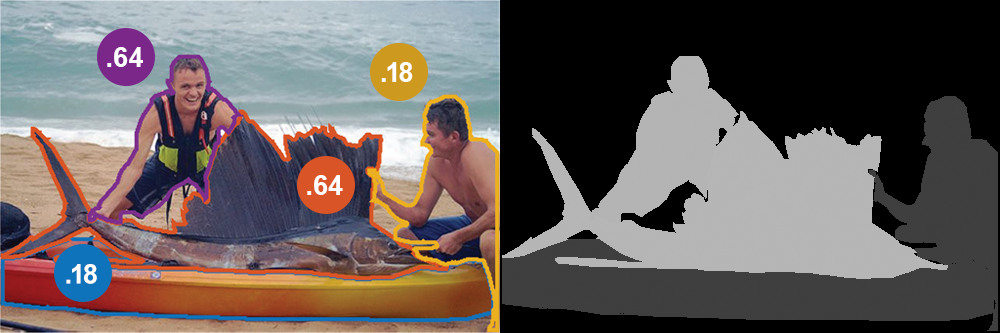
\includegraphics[width=0.475\textwidth]{figures/introduction/front_page.png}}
\vspace{-12pt}\caption{\footnotesize\textbf{Not all objects are equally remembered.} Image showing objects and their respective memorability scores (left) obtained from our experiment. We note that certain objects (the fish and left person) are more memorable than other objects. Right panel shows the ground truth map generated from the object segments and memorability scores.}\label{fig:introPhoto}%\vspace{-15pt}
\end{figure}

\begin{figure*}[!htb]
\centering
\subfigure{\centering 
\includegraphics[width=1\textwidth]{figures/method/main-task_v4.png}}
\vspace{-5mm}\caption{\footnotesize\textbf{Object Memory Game.} Participants viewed a series of images, followed by a sequence of objects and were asked to indicate whether each object was seen in the earlier sequence of full images. }\label{fig:mainTask}%\vspace{-12pt}
\end{figure*}

One of the primary goals of computer vision is to aid human-relevant tasks, such as object recognition, object detection, and scene understanding. Much of the algorithms in service of this goal have to make inferences about all objects in a scene. In comparison, humans are incredibly selective in the information they consider from the possible visual candidates they experience, and as a result, many human tasks are dependent on this filtering mechanism to be performed effectively. For this reason, it is important for vision systems to have information on hand concerning what objects humans deem important in the world, or in our specific case, which of them are worth remembering. Such information holds exciting promise. For example, it can enrich instructional designs for education, so as to maximize a student's retention while minimizing distractions, or enable intelligent ad placement software that embeds adverts in images and videos in such a way that humans are likely not to forget.

Going back to Figure \ref{fig:introPhoto}, why are the fish and left person more memorable and how do these objects influence the overall memorability of the photo? The field has made great strides in understanding comparable visual  properties of the world such as saliency \cite{it} and importance \cite{berg12}, but we still do not have a clear understanding of what objects are ``worth” remembering in the world. Although recent studies related to image memorability \cite{isola11,isola11nips,khosla13,isola14,zoya15} have explored this at the image-level, no work has explored what exactly in an image is remembered. Using object annotations and predictive models, such knowledge can be potentially inferred from the memorability score of an image alone \cite{khosla12}, but these methods will ultimately require ground truth object memorability data to be properly evaluated and analyzed. To enable the development of such approaches, we collect ground truth object-level memorability scores and conduct an extensive empirical investigation of  memorability at the object-level, a simple yet powerful strategy that provides detailed answers to many interesting questions at hand. While image memorability studies have provided invaluable knowledge, the study of object memorability in images not only sheds light on what elements of an image are remembered, but it also should eventually put forth, by its very nature, a bottom-up account of memorability. More importantly, such an analysis will enable unique applications in the fields of computer vision and computational photography not possible from the study of image memorability alone.

In this paper, we systematically explore the memorability of objects within individual images and shed light on the various factors that drive object memorability. In exploring the connection between object memorability, saliency, object categories, and image memorability, our paper makes several important contributions.

\vspace{3pt}\noindent\textbf{Contributions.} \textbf{(1)} This paper presents the first work that studies the problem of object memorability and provides a deeper understanding of what makes objects in an image memorable or forgettable. While previous work has tried to infer such knowledge  computationally \cite{khosla12}, our work is the first to directly quantify and study what objects in an image humans actually remember.  \textbf{(2)} We uncover the relationship between visual saliency and object memorability and demonstrate those instances where visual saliency directly predicts object memorability and when/why it fails to do so. While there have been a few very recent studies that explore the connection between image memorability and visual saliency \cite{zoya15,lemeur13,kim13}, our work is the first to explore the connection between object-level memorability and visual saliency. %To the best of our knowledge, our work is the first to show the differences and overlap between saliency and memorability and how the two phenomena differ from each other.
\textbf{(3)} We make significant headway in disambiguating the link between image and object memorability. We show that in many cases, the memorability of an image is primarily driven by the memorability of its most memorable object. %Studying these questions helps us not only understand visual saliency, image and object memorability in more detail, but it can also have important contributions to computer vision. For example, understanding which regions and objects in an image are memorable would enable us to modify the memorability of images which can have applications in advertising, user interface design, etc.
Furthermore, we show that our compiled dataset can serve as a benchmark for evaluating automated object memorability algorithms and enable/encourage future work in this exciting line of research.%object and region memorability prediction schemes.


\section{Measuring Object Memorability}

\begin{figure*}[!htb]
\centering
\subfigure{\centering 
\includegraphics[width=1\textwidth]{figures/method/main-task_v4.png}}
\vspace{-5mm}\caption{\footnotesize\textbf{Object Memory Game.} Participants viewed a series of images, followed by a sequence of objects and were asked to indicate whether each object was seen in the earlier sequence of full images. }\label{fig:mainTask}
\end{figure*}


As a first step towards understanding memorability of objects in
images, we compile an image database containing a variety of objects
from a diverse range of categories, as well as, measure the
probability that every object in each database image will be
remembered by a large group of subjects after a single viewing. 
%
This
helps provide ground truth memorability scores for objects inside
images (defined as image segments) and allows for a precise analysis
of the memorable elements within an image. 
%
Toward this, we utilized the
PASCAL-S dataset \cite{yin14}, a fully segmented dataset built on the
validation set of the PASCAL VOC 2010 \cite{pascal10} segmentation
challenge. To improve segmentation quality, we manually refined the
segmentations from this dataset. We removed all homogenous non-object
or background segments (e.g. ground, grass, floor, and sky), along
with, imperceptible object fragments and excessively blurred
regions. All remaining object segmentations were tested for
memorability. In summary, our final dataset comprises $850$ images and
$3,412$ object segmentations (i.e. an average of $4$ objects per
image), for which we gathered ground truth memorability through crowd
sourcing. %\B{how about image size? - they were all in their original
          %sizes and aspect ratios.} 


\subsection{Object Memory Game}
To measure the memorability of individual objects in each dataset image %\B{use either database or dataset consistently throughout the paper}
, we created an alternate version of the Visual Memory Game through Amazon Mechanical Turk following the basic design in \cite{isola11}, with the exception of a few key differences (refer to Figure \ref{fig:mainTask}). In our game, participants first viewed a sequence of $35$ images one at a time, with a $1.5$ second interval between image presentations. The subjects were asked to remember the contents and objects inside these images as much as they could. To ensure that subjects would not only just  look at the salient or center objects, they were given unlimited time to freely view the images. Once they were done viewing an image, they could press any key to advance to the next image. After the initial image sequence, participants viewed a sequence of $45$ objects, their task then being to indicate through a key press which of those objects was present in one of the previously shown images. Each object was displayed for $1.5$ seconds, with a $1.5$ second gap in between each object in the sequence. Pairs of corresponding image and object sequences were broken up into $10$ blocks. Each block consisted of $80$ total stimuli ($35$ images and $45$ objects), and lasted approximately $3$ minutes. At the end of each block, the subject could take a short break. Overall, the experiment takes approximately $30$ minutes to complete.

Unknown to the subjects, each sequence of images inside each block was pseudo-randomly generated to consist of $3$ ``target'' images taken from the Pascal-S dataset, whose objects were later presented to the participants for identification. The remaining images in the sequence consisted of $16$ ``filler'' images and $16$ ``familiar'' images. 
Filler images were randomly selected from the DUT-OMRON dataset \cite{dutomron13}, while the familiar ones were randomly sampled from the MSRA dataset \cite{msra11}. In a similar fashion, the object sequence in each block was also generated pseudo-randomly to consist of $3$ target objects ($1$ object taken randomly from each previously shown target image). The remaining objects in the sequence consisted of $10$ control, $16$ filler, and $16$ familiar objects. Filler objects were sampled randomly from the $80$ different object categories in the Microsoft COCO dataset \cite{coco14}, while the familiar objects were sampled from objects taken from the previously displayed familiar images in the image sequence. The fillers and familiars helped provide spacing between the target images and target objects, whereas the control objects allowed us to check if the subjects were paying attention to the task \cite{brady08,isola11}. While the fillers and familiars (both images and objects) were taken from datasets of real world scenes and objects, the control objects were artificial stimuli randomly sampled from the dataset proposed in \cite{brady08} and served as a control to test subject attentiveness. Target images and their corresponding target objects were spaced $70-79$ stimuli apart, while familiar images and their objects were spaced $1-79$ stimuli apart. All images and objects appeared only once, and each subject was tested on only one object from each target image. Objects were centered within the image they originated from and non-object pixels were set to grey. Participants were required to complete the entire task, which included $10$ blocks ($\sim$$30$ minutes) and could not participate in the experiment a second time. After collecting the data, we assign a memorability score to each target object in our dataset, defined as the percentage of correct detections by subjects (refer to Figure \ref{fig:introPhoto} for an example). In all our analysis, we remove all subjects whose accuracy on the control objects is below $70\%$. In the end, this memorability game had a total of $1,823$ workers from Mechanical Turk with more than $95\%$ approval rating in Amazon’s system. The memorability score of an object corresponds to the number of subjects that correctly detected the presence of that object in a previously seen image. On average, each object was scored by $16$ subjects and the average memorability score was $33\%$ with a standard deviation of  $28\%$. %\B{Is this a large deviation? does it need explanation? no I don't think so.. some objects were barely memorable and some of them had a high memorability}.   


\subsection{Consistency Analysis}
%Previous work on image memorability has found human consistency to be fairly high. That is, people tend to remember the same images, and exhibit similar performance in doing so. Despite variability due to individual differences and other sources of noise, this level of consistency provides evidence that memorability is an intrinsic property of images that can be predicted. In contrast to full images, this paper focuses primarily on the memorability of individual objects in an image, which may or may not exhibit the same level of human consistency as full images, which often contain complex arrangements of several objects. High consistency in object memorability would indicate that, like full images, objects can potentially be predicted with high accuracy.
To assess human consistency in remembering objects, we repeatedly divided our entire subject pool into two equal halves and quantified the degree to which memorability scores for the two sets of subjects were in agreement using Spearman’s rank correlation ($\rho$). We computed the average correlation over $25$ of these random split iterations, yielding an average correlation of $\rho=0.76$. This high consistency in object memorability indicates that, like full images, object memorability is a shared property across subjects. People tend to remember (and forget) the same objects in images, and exhibit similar performance in doing so. Thus memorability of objects in images can potentially be predicted with high accuracy. In the next section, we study the various factors that possibly drive object memorability in images.

%this level of
%consistency suggests that information intrinsic to the images
%might be used by different people to remember them.
%In the next section, we search for this image information.



\section{Understanding Object Memorability}

In this section, we aim to better understand object memorability and the factors that make an object more memorable or forgettable to humans. We first investigate the role that simple color features play in determining object memorability.

\subsection{Can simple features explain memorability?}

\begin{figure}[!htb]
\centering
\subfigure{\centering \includegraphics[width=0.47\textwidth]{figures/results/simple_features/color_corrs.png}}
\vspace{-5mm}\caption{\footnotesize\textbf{Simple color features do not explain object memorability.} Correlations of object memorability scores with hue and saturation are near zero, and only value shows a very weak correlation.}\label{fig:simple}
\end{figure}

While simple low-level image features are traditionally poor
predictors of image memorability \cite{isola11} (with good reason
\cite{konkle10}), the question arises whether such features play any
role in determining object memorability in images. To address this
query and following a similar strategy as in \cite{isola11,isola14},
we compute the mean (and variance) of HSV color of each object in our
dataset, i.e. first and second order  statistics of pixel color within
an object's ground truth segmentation, and correlate it (Spearman rank
correlation) with the underlying object memorability score (refer to
Figure \ref{fig:simple}). We see that the mean ($\rho = 0.1$) and
variance ($\rho=0.25$) of the V channel show weak correlation with
object memorability, suggesting that brighter and higher contrast
objects may be more memorable. On the other hand, essentially no
relationship exists between memorability and either the H or S
channels. This slightly deviates from the findings in \cite{isola11},
which show mean hue to be weakly predictive of image
memorability. This difference could be due to the fact that many
images of the dataset in \cite{isola11} show blue and green outdoor
landscapes as being less memorable than warmly colored human faces and
indoor scenes, while our dataset contains plenty of indoor objects and
people and outdoor scene-related segments such as sky and ground are
not included as objects. From these results, we see that, like image
memorability, simple pixel statistics do not play a significant role
in determining object memorability in images.



\subsection{What is the role of saliency in memorability?}

Intuitively, the regions within an image that are most salient are likely to have a higher probability of being remembered, since they will draw the attention of viewers and a majority of a viewer’s eye fixations will be spent looking at those regions.. On the other hand, it is conceivable that some visually appealing regions will not be memorable, especially since aesthetic images are known to be less memorable \cite{isola11}, \cite{isola14}. When can visual saliency predict object memorability and what are the possible differences between these two phenomena? Quantifying the precise relationship between saliency and memorability will be paramount  towards understanding object memorability in greater depth.

To this aim, we utilized the eye fixation dataset made available for the Pascal-S dataset in \cite{yin14}. With this dataset in hand, we first calculated the number of unique fixation points within the area of each object and computed the correlation between this metric and the object’s memorability score (Figure \ref{fig:scatterFixation} a). We found this correlation to be positive and considerably high ($\rho = 0.71$), suggesting that fixation count and visual saliency may drive object memorability considerably. However, the large concentration of points on the bottom left part of scatter plot in Figure \ref{fig:scatterFixation} a suggests that part of the reason for this high correlation is that objects that have not been viewed at all have essentially no memorability. Indeed, only objects that have been seen can be remembered. In addition, the points toward the top left appear to decrease in trend. Looking deeper, Figure \ref{fig:fixCorr} plots the change in correlation between object memorability and fixations as the minimum number of fixations inside objects increases. The downward monotonic trend indicates that as the number of fixations inside an object increases, the predictive ability diminishes significantly. In addition, Figure \ref{fig:fixCorr} plots the correlation between object memorability and number of fixations as a function of total number of objects in an image. Similar to the previous trend, as the number of objects in an image increases, the correlation between saliency i.e. number of fixations and memorability score decreases sharply. This finding is in agreement with the two remaining scatter plots in Figure \ref{fig:scatterFixation} b (shows that the memorability of an object decreases in the presence of many other objects) and Figure \ref{fig:scatterFixation} c (shows that number of fixations decreases with the number of objects). This makes intuitive sense since people have more to look at in an image when more objects are present, and so they may look less at any one object, especially if they compete for saliency, and therefore may have a more difficult time remembering those objects.

\begin{figure}[t]
\centering
\subfigure{\centering \includegraphics[width=0.5\textwidth]{figures/results/fixation/mem-fix-corr-by-factors.png}}
\vspace{-5mm}\caption{\footnotesize\textbf{Correlation between object memorability and number of fixations.} add-in later. }\label{fig:fixCorr}
\end{figure}

To sum up, saliency is a surprisingly good index of object memorability in simple contexts where there are few objects in the image, or when an object has few interesting points, but it is a much weaker predictor of object memorability in complex scenes containing multiple objects that have many points of interest (Figure \ref{fig:fixQual}).

\begin{figure}[b]
\centering
\subfigure{\centering \includegraphics[width=0.5\textwidth]{figures/results/fixation/fix_corr_set.png}}
\vspace{-5mm}\caption{\footnotesize\textbf{Correlation between object memorability and number of fixations.} add-in later. }\label{fig:scatterFixation}
\end{figure}

\textbf{Center Bias: } Figure \ref{fig:fixPos} elucidates another example where saliency and memorability diverge. Previous studies related to visual saliency have showed that saliency is heavily influenced by center bias \cite{judd09}, \cite{sun08}, primarily due to photographer bias (also evident from the leftmost plot in Figure \ref{fig:fixPos}) and viewing strategy \cite{tseng2009}. Since our data collection experiment tries to control for the viewing strategy, memorability exhibits comparatively less center bias than saliency. This is most apparent when considering the difference in the solid ellipse in the right plot (shows where $95\%$ of fixation positions are located), and the dashed ellipse (shows where the $95\%$ of the above-median memorable objects are located).

%Our work serves as the first direct evidence that saliency and memorability differ from each other by exploring the differences and overlap between the two.
%To the best of our knowledge, our work is the first to show the differences and overlap between saliency and memorability and how the two phenomena differ from each other.

\begin{figure}[t]
\centering
\subfigure{\centering \includegraphics[width=0.45\textwidth]{figures/results/fixation/positions_final.png}}
\vspace{-5mm}\caption{\footnotesize\textbf{Positions.} add-in later. }\label{fig:fixPos}
\end{figure}

\begin{figure}[t]
\centering
\subfigure{\centering \includegraphics[width=0.45\textwidth]{figures/results/fixation/qual/qual.png}}
\vspace{-5mm}\caption{\footnotesize\textbf{Saliency Fail cases.} add-in later. }\label{fig:fixQual}
\end{figure}


 \label{sec:fix}

\subsection{How do object categories affect memorability?}

In the previous section, we explored the relationship between visual saliency of an object and its memorability. Now, we explore how an object's category influences the probability that it will be remembered.

\subsubsection{Are some object categories more memorable?}

For this analysis, we had three in-house annotators manually label the object segmentations in our dataset. The annotators were provided the original image (for reference) and the object segmentation and asked to assign a single category to the segment out of $7$ possible categories: animal, building, device, furniture, nature, person, and vehicle. We chose these categories so that a wide range of object classes could be covered. For example, category ``device” includes objects like utensils, bottles, and televisions, while ``nature” includes objects like trees, mountains, and flowers, and “vehicle” contains cars, bikes, and airplanes. Figure \ref{fig:avgMem} shows the distribution of the memorability scores of all $7$ object categories in our dataset.

\begin{figure}[!htb]
\centering
\subfigure{\centering \includegraphics[width=0.45\textwidth]{figures/results/obLabel/memScore_dist2.png}}
\vspace{-5mm}\caption{\footnotesize\textbf{Average memorability per object class.} Figure showing some object classes are more memorable than others. }\label{fig:avgMem}
\end{figure}

Results in Figure \ref{fig:avgMem} give a sense of how  memorability changes across different object categories. Animal, person, and vehicle are all highly memorable classes each associated with  an average memorability score greater than or close to $0.5$. Interestingly, all other categories have an average memorability lower than $0.25$, indicating that humans do not remember objects from these categories very well. In particular, furniture is the least memorable category with an average score of only $0.14$. This is possibly due to the fact that most objects in the furniture, nature, and building categories either appear mostly in the background or are occluded, which likely decreases their memorability significantly. In contrast, objects from the animal, person, and vehicle categories appear mostly in the foreground, leading to a higher memorability score on average. Interestingly, the most memorable objects from building, furniture, and nature tend to have an average memorability in the range of $0.4 - 0.8$, whereas the score of the most memorable objects from person, animal and vehicle is higher than $0.9$. %This is particularly interesting as these top objects are not occluded and most of them tend to appear in the foreground. 
While the differences in the memorability of different object categories could be driven due to factors like occlusion, size, background/foreground, or photographic bias, the distribution in Figure \ref{fig:avgMem} suggests that humans remember some object classes such as person, animal, and vehicle irrespective of external nuisance factors and these categories are \textit{intrinsically} more memorable than others.


%distribution of the most memorable objects within each class suggest that memorability could be an intrinsic property of an object class.  The right side of the figure presents an interesting analysis This analysis is particularly interesting as these top objects are not occluded and most of them tend to appear in the foreground. The top $20$ most memorable objects from person, animal and vehicle have memorability higher than $0.90$ whereas the average memorability of the top $20$ objects from building, furniture, and nature is lesser than $0.70$. While the differences in the memorability of different classes could be driven primarily due to factors like occlusion, size, background/foreground, the results in table \ref{tab:avgMem} suggest that memorability could be an intrinsic property of an object class and some object classes like person, animal, vehicle are in general intrinsically more memorable than classes like furniture, nature etc.
%



\subsubsection{Exploring category-specific memorability}


\begin{figure*}[!htb]
\centering
\subfigure{\centering 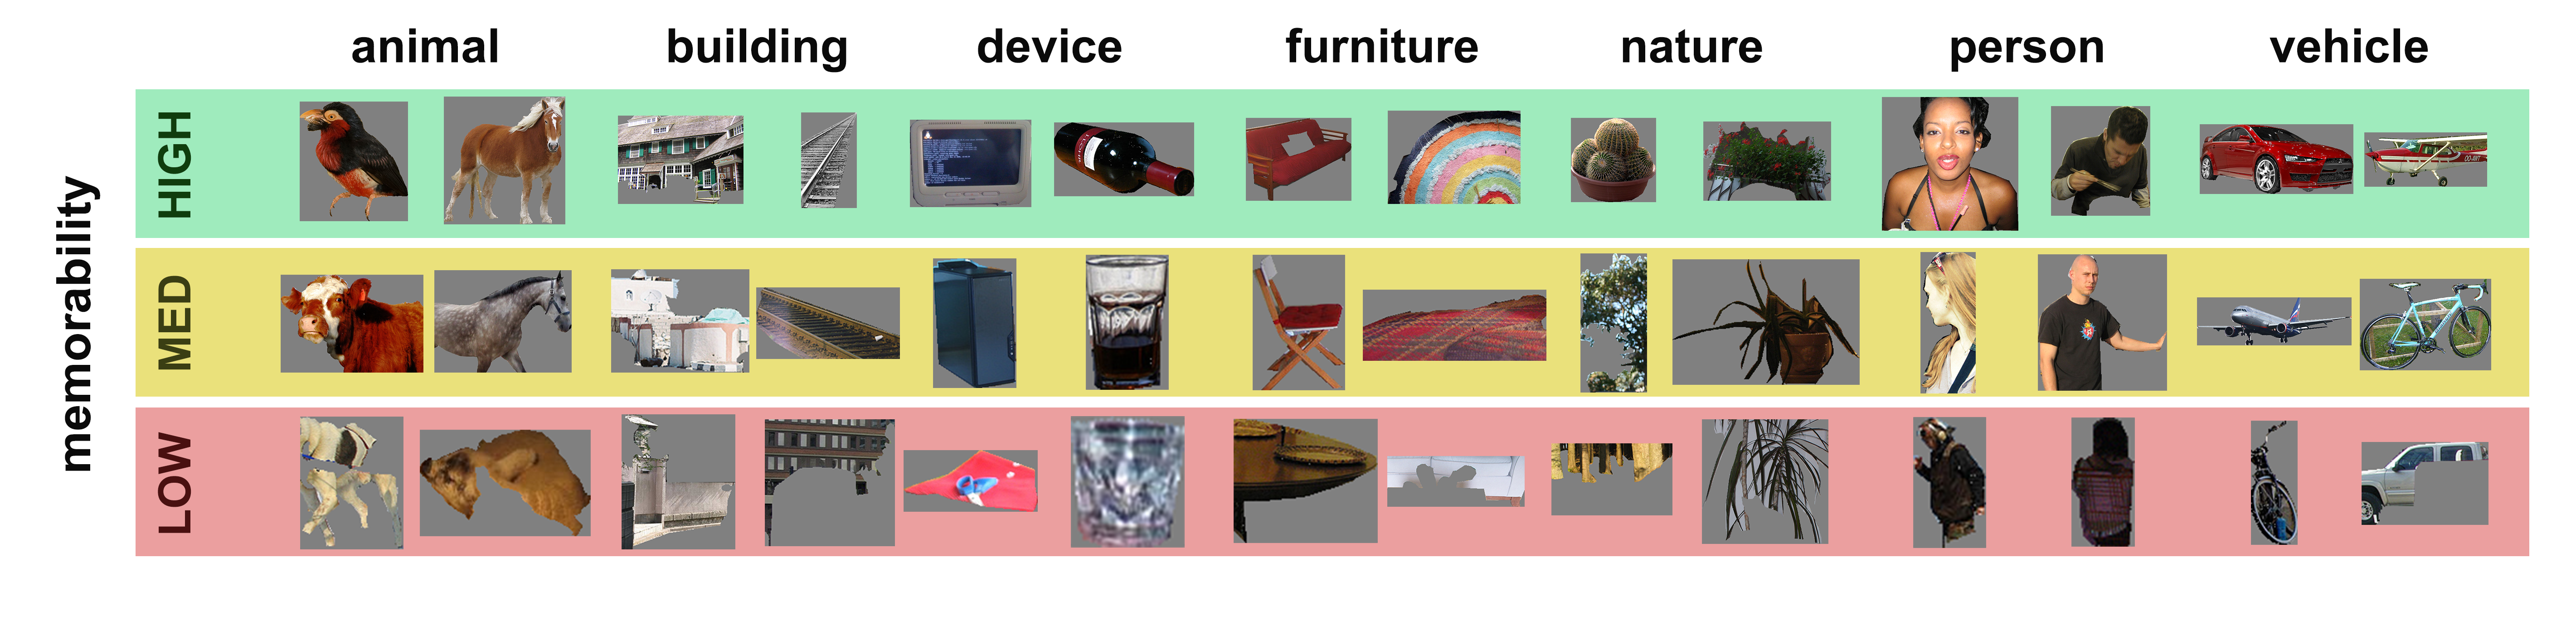
\includegraphics[width=1\textwidth]{figures/results/obLabel/qual_cat_v2.png}}
\vspace{-24pt}\caption{\footnotesize\textbf{Memorability of object categories.} Most memorable, medium memorable and least memorable objects from each of the $7$ categories.}\label{fig:obLabelQual}%\vspace{-12pt}
\end{figure*}

As demonstrated above, some object categories (i.e. animal, person, and vehicle) tend to be more memorable than others. However, not all objects in the same category are equally memorable. The examples in Figure \ref{fig:obLabelQual} show the most memorable, medium memorable, and least memorable objects for each category. Across categories, non-memorable objects tend to be those that are occluded and obstructed by other objects. What other category-related factors could influence the memorability of objects? Among the possible factors, we explore how category-specific object memorability is influenced by \textbf{(i)} the number of objects in an image and \textbf{(ii)} the presence of other object categories.


\vspace{3pt}\noindent\textbf{Number of objects:} %We first examined how the memorability of each object class is affected by the number of objects inside an image.
Figure \ref{fig:obLabelChange} shows the change in average memorability for the different categories when the minimum number of objects within an image is increased. Results indicate that the number of objects present in an image is an important factor in determining memorability. For example, as the number of objects in an image increases, the memorability of animals and vehicles decreases sharply, most likely as a result of competition for attention. Interestingly, the memorability of the person category does not change significantly when an increasing number of objects exist in the image. This suggests that people are not only one of the most memorable object categories, but that their memorability is the least sensitive to the presence of object clutter in an image. This may be because a single person steals most of the viewer's attention in an image, but how is this behavior characterized in the presence of other multiple people in the same image? To answer this, we turn to the question of interclass memorability next.

\begin{figure}[!t]
\centering
\subfigure{\centering \includegraphics[width=0.47\textwidth]{figures/results/obLabel/memScore_change2.png}}
\vspace{-5mm}\caption{\footnotesize\textbf{Object number affects category-specific memorability.} For each category, a curve is plotted that shows the change in average memorability with an increase in the number of objects. The memorability of objects belonging to categories like animals and vehicles goes down significantly with an increase in object number.}\label{fig:obLabelChange}
\end{figure}

\begin{figure}[!b]
\centering
\subfigure{\centering 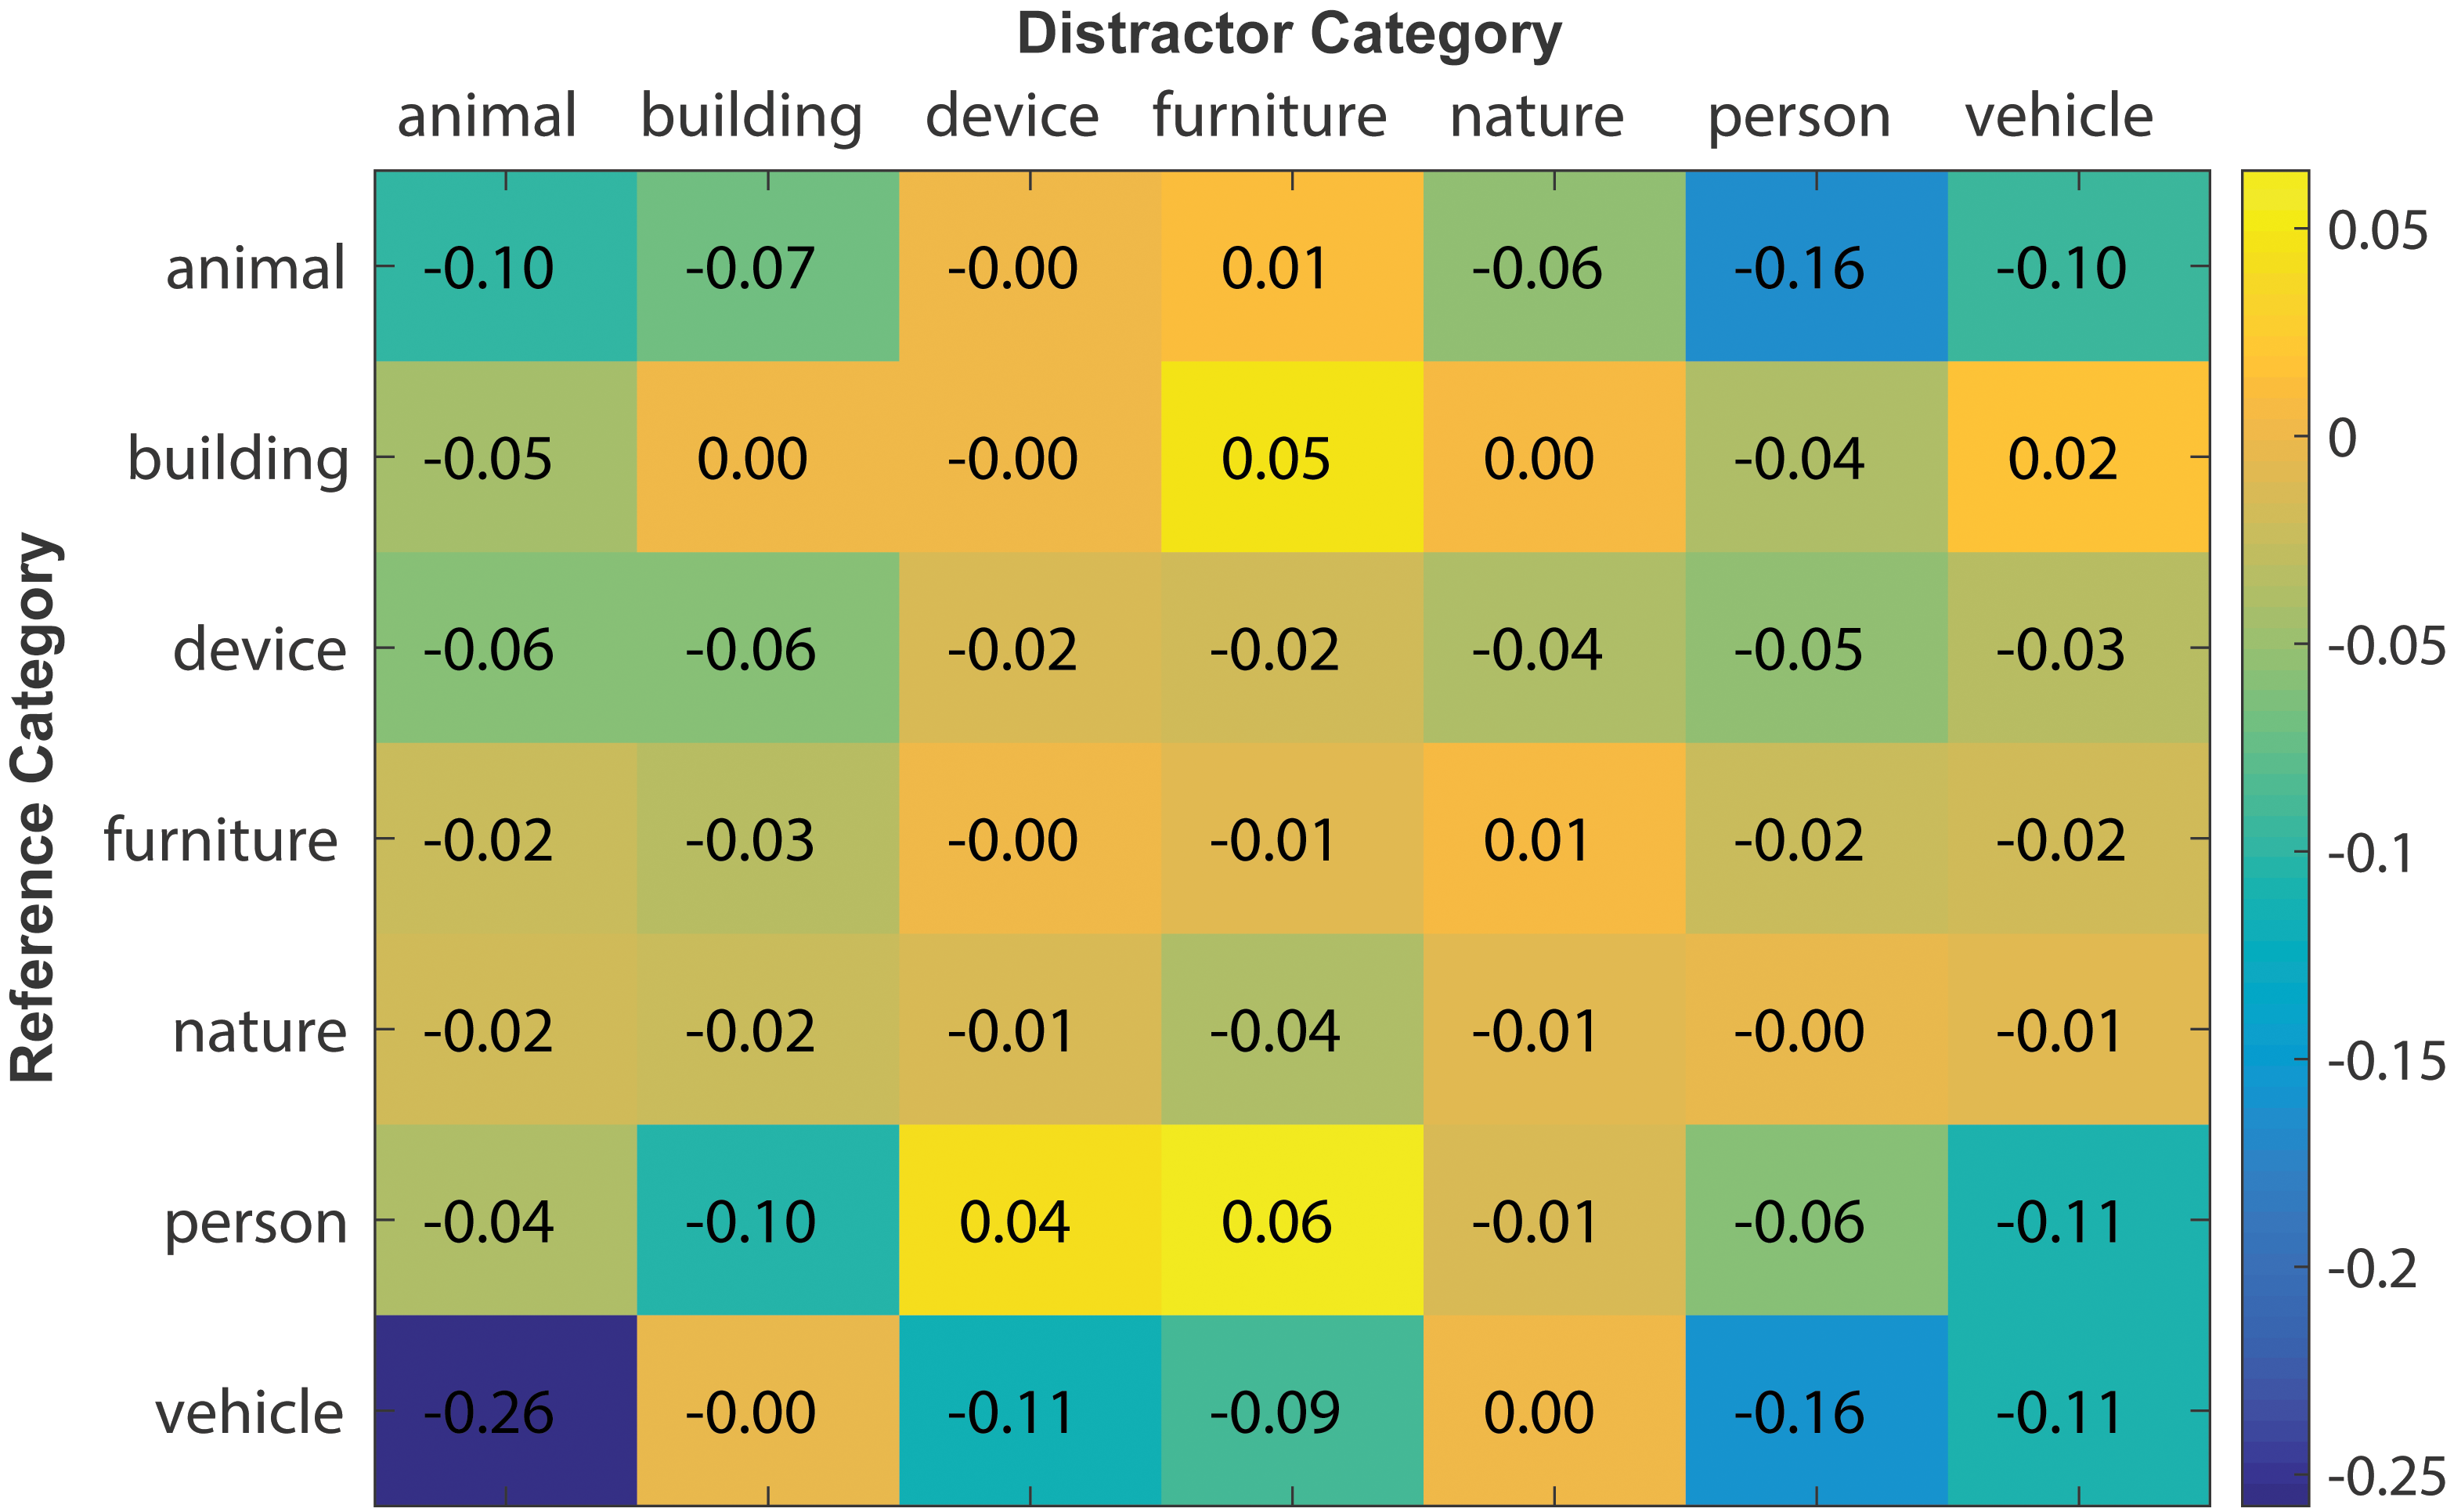
\includegraphics[width=0.47\textwidth]{figures/results/obLabel/confusionMatrix_v2.png}}
\vspace{-5mm}\caption{\footnotesize\textbf{Inter-class object memorability relationship.} The effect on memorability a distractor category has on each reference category }\label{fig:obLabelPair}
\end{figure}

\vspace{3pt}\noindent\textbf{Inter-class memorability:} How much is the memorability of a particular object category affected when it co-occurs with another object category (or another instance of the same category)? To quantify the effect of one category on another, we consider each pairwise combination of categories and gather all images that contain at least one object from both categories. By taking one category as the \emph{reference} and the other as the \emph{distractor}, we compute the average memorability score $m_{R|D}$ of the reference in the  images common to the reference and distractor. To isolate the effect of the distractor, we compute the memorability difference $\Delta m=(m_{R|D}-m_R)$, where $m_R$ is the memorability score of the reference in all images where it exists. Figure \ref{fig:obLabelPair} shows $\Delta m$ for all possible reference and distractor pairs. It is clear that  $\Delta m$ for low-memorability categories (i.e. nature, furniture, device, and building) is not significantly affected by the presence of other categories. %Instead, their memorability tends to remain low across all contexts.



Also, the memorability of the animal category maintains its high score in the presence of other categories, except vehicles, people, and itself, where it decreases substantially. The memorability of people tends to be unaffected by the presence of most other categories including itself. However, it decreases in the presence of vehicles and buildings. This could be due to the fact that people in images containing vehicles or buildings are usually zoomed out and smaller in size (refer to Figure \ref{fig:qualInterClass}). The memorability of the vehicle category is strongly affected by the presence of other object categories. In particular, it drops significantly in the presence of another vehicle, people, and animals.


\begin{figure}[t]
\centering
\subfigure{\centering \includegraphics[height = 1.1 cm]{figures/results/obLabel/inter-class/14.jpg}}
\subfigure{\centering \includegraphics[height = 1.1 cm]{figures/results/obLabel/inter-class/85.jpg}}
\subfigure{\centering \includegraphics[height = 1.1 cm]{figures/results/obLabel/inter-class/10.jpg}}
\subfigure{\centering \includegraphics[height = 1.1 cm]{figures/results/obLabel/inter-class/128.jpg}}
\subfigure{\centering \includegraphics[height = 1.1 cm]{figures/results/obLabel/inter-class/102.jpg}}
\subfigure{\centering \includegraphics[height = 1.1 cm]{figures/results/obLabel/inter-class/129.jpg}}\\
\vspace{-2mm}
\subfigure{\centering \includegraphics[height = 1.1 cm]{figures/results/obLabel/inter-class/14.png}}
\subfigure{\centering \includegraphics[height = 1.1 cm]{figures/results/obLabel/inter-class/85.png}}
\subfigure{\centering \includegraphics[height = 1.1 cm]{figures/results/obLabel/inter-class/10.png}}
\subfigure{\centering \includegraphics[height = 1.1 cm]{figures/results/obLabel/inter-class/128.png}}
\subfigure{\centering \includegraphics[height = 1.1 cm]{figures/results/obLabel/inter-class/102.png}}
\subfigure{\centering \includegraphics[height = 1.1 cm]{figures/results/obLabel/inter-class/129.png}}
\vspace{-5mm}\caption{\footnotesize\textbf{Memorability of person in presence of other categories.} Top row: Images where a person co-occurs with other categories. Bottom row: Ground truth object memorability maps. In the presence of buildings, the memorability of person can drop. In the presence of a vehicle or animal, the person usually is more memorable. }\label{fig:qualInterClass}
\end{figure}

In summary, when an animal, vehicle or a person co-occur in the same image, the memorability of all three categories usually decreases. However, this pattern of change in memorability is category-specific in general. For example, when a vehicle and animal are present in the same image, the animal is generally more memorable, even though both their memorability scores drop significantly. When a vehicle or an animal co-occurs with a person, the person is generally more memorable (also shown in Figure \ref{fig:qualInterClass}).









\subsection{How are object \& image memorability related?}

\begin{figure*}[!thb]
\centering
\subfigure{\centering \includegraphics[width=1\textwidth]{figures/results/imMem/qual.png}}
\vspace{-16pt}\caption{\footnotesize\textbf{Max object memorability predicts image memorability.} Top row: most memorable images taken from our dataset along with their highest memorable object and their respective memorability scores. Bottom row: least memorable images in the dataset along with their most memorable object and their respective memorability scores. We notice that the maximum object memorability correlates strongly with image memorability in both the cases. }\label{fig:imMemQual}%\vspace{-12pt}
\end{figure*}

Until now, we have studied what objects people remember and the factors that influence their memorability, but to what extent does the memorability of individual objects affect the overall memorability of an image? Moreover, if an image is highly memorable, what can we say about the memorability of the objects inside those images (and vice versa)? To shed light on these queries, we conducted a second large-scale experiment on Amazon Mechanical Turk for all images in our dataset to gather their respective \emph{image} memorability scores. For this experiment, we followed the same strategy as the memory game experiment proposed in \cite{isola11}. A series of images from our dataset and Microsoft COCO dataset \cite{coco14} (i.e. `filler' images) were flashed for $1$ second each, and subjects were instructed to press a key whenever they detected a repeat presentation of an image. A total of $350$ workers participated in this experiment with each image being viewed $80$ times on average. The rank correlation after averaging over $25$ random splits was $0.7$, thus, validating annotator consistency in  the image memorability scores.






Using results from the previous experiments, we computed the correlation between the scores of the single most memorable \emph{object} in each image and the memorability score of each \emph{image}. This correlation is moderately high with $\rho=0.4$, suggesting that the most memorable object in an  image plays a crucial role in determining the overall memorability of an image. To investigate this finding in relation to some extreme cases, we repeated the same analysis as above but on a subset of the data containing the $100$ most memorable images and the $100$ least memorable images. The correlation between maximum object memorability and image memorability for this subset of images increased significantly to $\rho=0.62$. This means that maximum object memorability serves as a strong indicator of whether an image is \textit{highly} memorable or \emph{not} memorable at all. In other words, images that are highly memorable contain at least one highly memorable object and images with low memorability usually do not contain a single highly memorable object (refer to Figure \ref{fig:imMemQual}).

It seems that maximum object memorability is highly explanatory, but does this behavior generalize across object categories? We further computed the correlation between maximum object and image memorability for each individual object category. The correlation for the categories were: animal ($\rho=0.38$), building ($\rho=0.22$), device ($\rho=0.47$), furniture ($\rho=0.53$), nature ($\rho=0.64$), person ($\rho=0.54$), and vehicle ($\rho=0.30$) which shows that certain categories are more strongly correlated than others. For example, images containing animals, buildings, or vehicles as the most memorable objects tend to have varying degree of image memorability (indicated by their lower $\rho$ values). On the other hand, device, furniture, nature, and person are strongly correlated with image memorability, indicating that if an image's most memorable object belongs to one of these categories, the object memorability score is strongly predictive of the image memorability score. We can imagine scenarios in which this information is potentially useful. For example, in vision systems that are tasked to predict scene memorability, a \textit{single} object and its category can serve as a strong prior in predicting this score.






 

\section{Predicting Object Memorability}

Although the primary goal of our paper is to \textit{understand} what drives memorability of objects in a scene, the current work also makes available the very first dataset containing the ground truth memorability of constituent objects from a highly diverse image set. In this section, we show that our dataset can serve as a  benchmark for the purpose of object memorability prediction by making use of the ground truth memorability maps constructed from experimental data.

\textbf{Baseline models:} As a first step, we propose a simple baseline model that utilizes a conv-net \cite{krizhevsky12}, \cite{jia14} trained on the ImageNet database \cite{deng09}. Since object categories play an important role in determining object memorability (\ref{sec:obLabel}), and deep learning models have recently been shown to achieve state-of-the-art results in various other recognition tasks, including object recognition and object categorization (cite papers here), we believe that this simple model can serve as a good initial baseline for object memorability prediction. We first generated object segments by using MCG, a generic object proposal method proposed in \cite{arbelaez14}. Next, we trained an SVR using $6$-fold cross-validation on the original segments to map deep features to memorability scores. We then used this model to predict the memorability scores for the top K ($K=20$) segments (obtained via the ranking scores provided by the MCG algorithm) for each image. After obtaining the predicted memorability scores, the memorability maps were generated by averaging the top $K$ segments at the pixel level. Since image features like SIFT \cite{lowe04} and HOG \cite{dalal05} have previously been shown to achieve good performance in predicting image memorability, we built a second baseline model using these features for comparison. Training and testing of this model was performed similar to the deep-net baseline model.

\textbf{Evaluation: } To evaluate the accuracy of the predicted memorability maps, we computed the rank correlation between the mean predicted memorability score inside each of the original object segments and their ground truth memorability scores. From figure \ref{fig:benchmark}, we first note that our deep-net baseline model performs considerably well ($\rho = 0.39$), reaching a level of performance that approaches  that of human consistency. In contrast, the baseline model trained using HOG and SIFT features exhibits much lower overall performance ($\rho = 0.27$). We also included $8$ state-of-the-art-saliency methods \textbf{gb} \cite{gb}, \textbf{aim} \cite{aim}, \textbf{dv} \cite{dv}, \textbf{it} \cite{it}, \textbf{gc} \cite{gc}, \textbf{pc} \cite{pc}, \textbf{sf} \cite{sf}, and \textbf{ft} \cite{ft} to our comparison (some of these are the top performing methods according to benchmarks in \cite{borji13}, \cite{borji12}). Saliency maps generated from these methods are likely to have some degree of overlap with memorability and are therefore worth comparing to our baseline, especially given the absence of alternative memorability prediction methods. Results from figure \ref{fig:benchmark}) show that the HOG+SIFT baseline is outperformed by most saliency methods. Thus, even though models using these features have previously demonstrated high predictive power in predicting image memorability, they may not be as well  suited for the task of predicting object memorability. The deep-net baseline model performs better than all other saliency methods and only \textbf{pc} ($\rho=0.38$), \textbf{sf} ($rho=0.37$), and \textbf{gb} ($rho=0.36$) show performance comparable to the model. A common factor between these saliency methods is that they explicitly add center bias to their implementation, which could be a  part of the reason for their favorable performance. Despite this, the deep-net model performs comparably against them and is potentially much better suited for memorability prediction. Thus, we recommend in the future, memorability algorithms compare their methods against our deep-net baseline. While the deep-net model performed fairly well, part of the performance of such a model is dependent on the quality of the segmentations used. For this reason, we also consider the upper bound of our current predictive power by showing the results for our model containing predictions on the original segments (Figure \ref{fig:benchmark}). Interestingly, the accuracy of this model is very high and close to human performance ($\rho = 0.7$). This demonstrates that the deep-net model has high predictive ability that is suppressed most heavily by constraints of the segmentation task. As the main insight of our evaluation, we have have demonstrated that deep features serve as strong predictors of memorability and selection of higher quality segments can potentially lead to improved memorability prediction algorithms.

\begin{figure}[t]
\centering
\subfigure{\centering 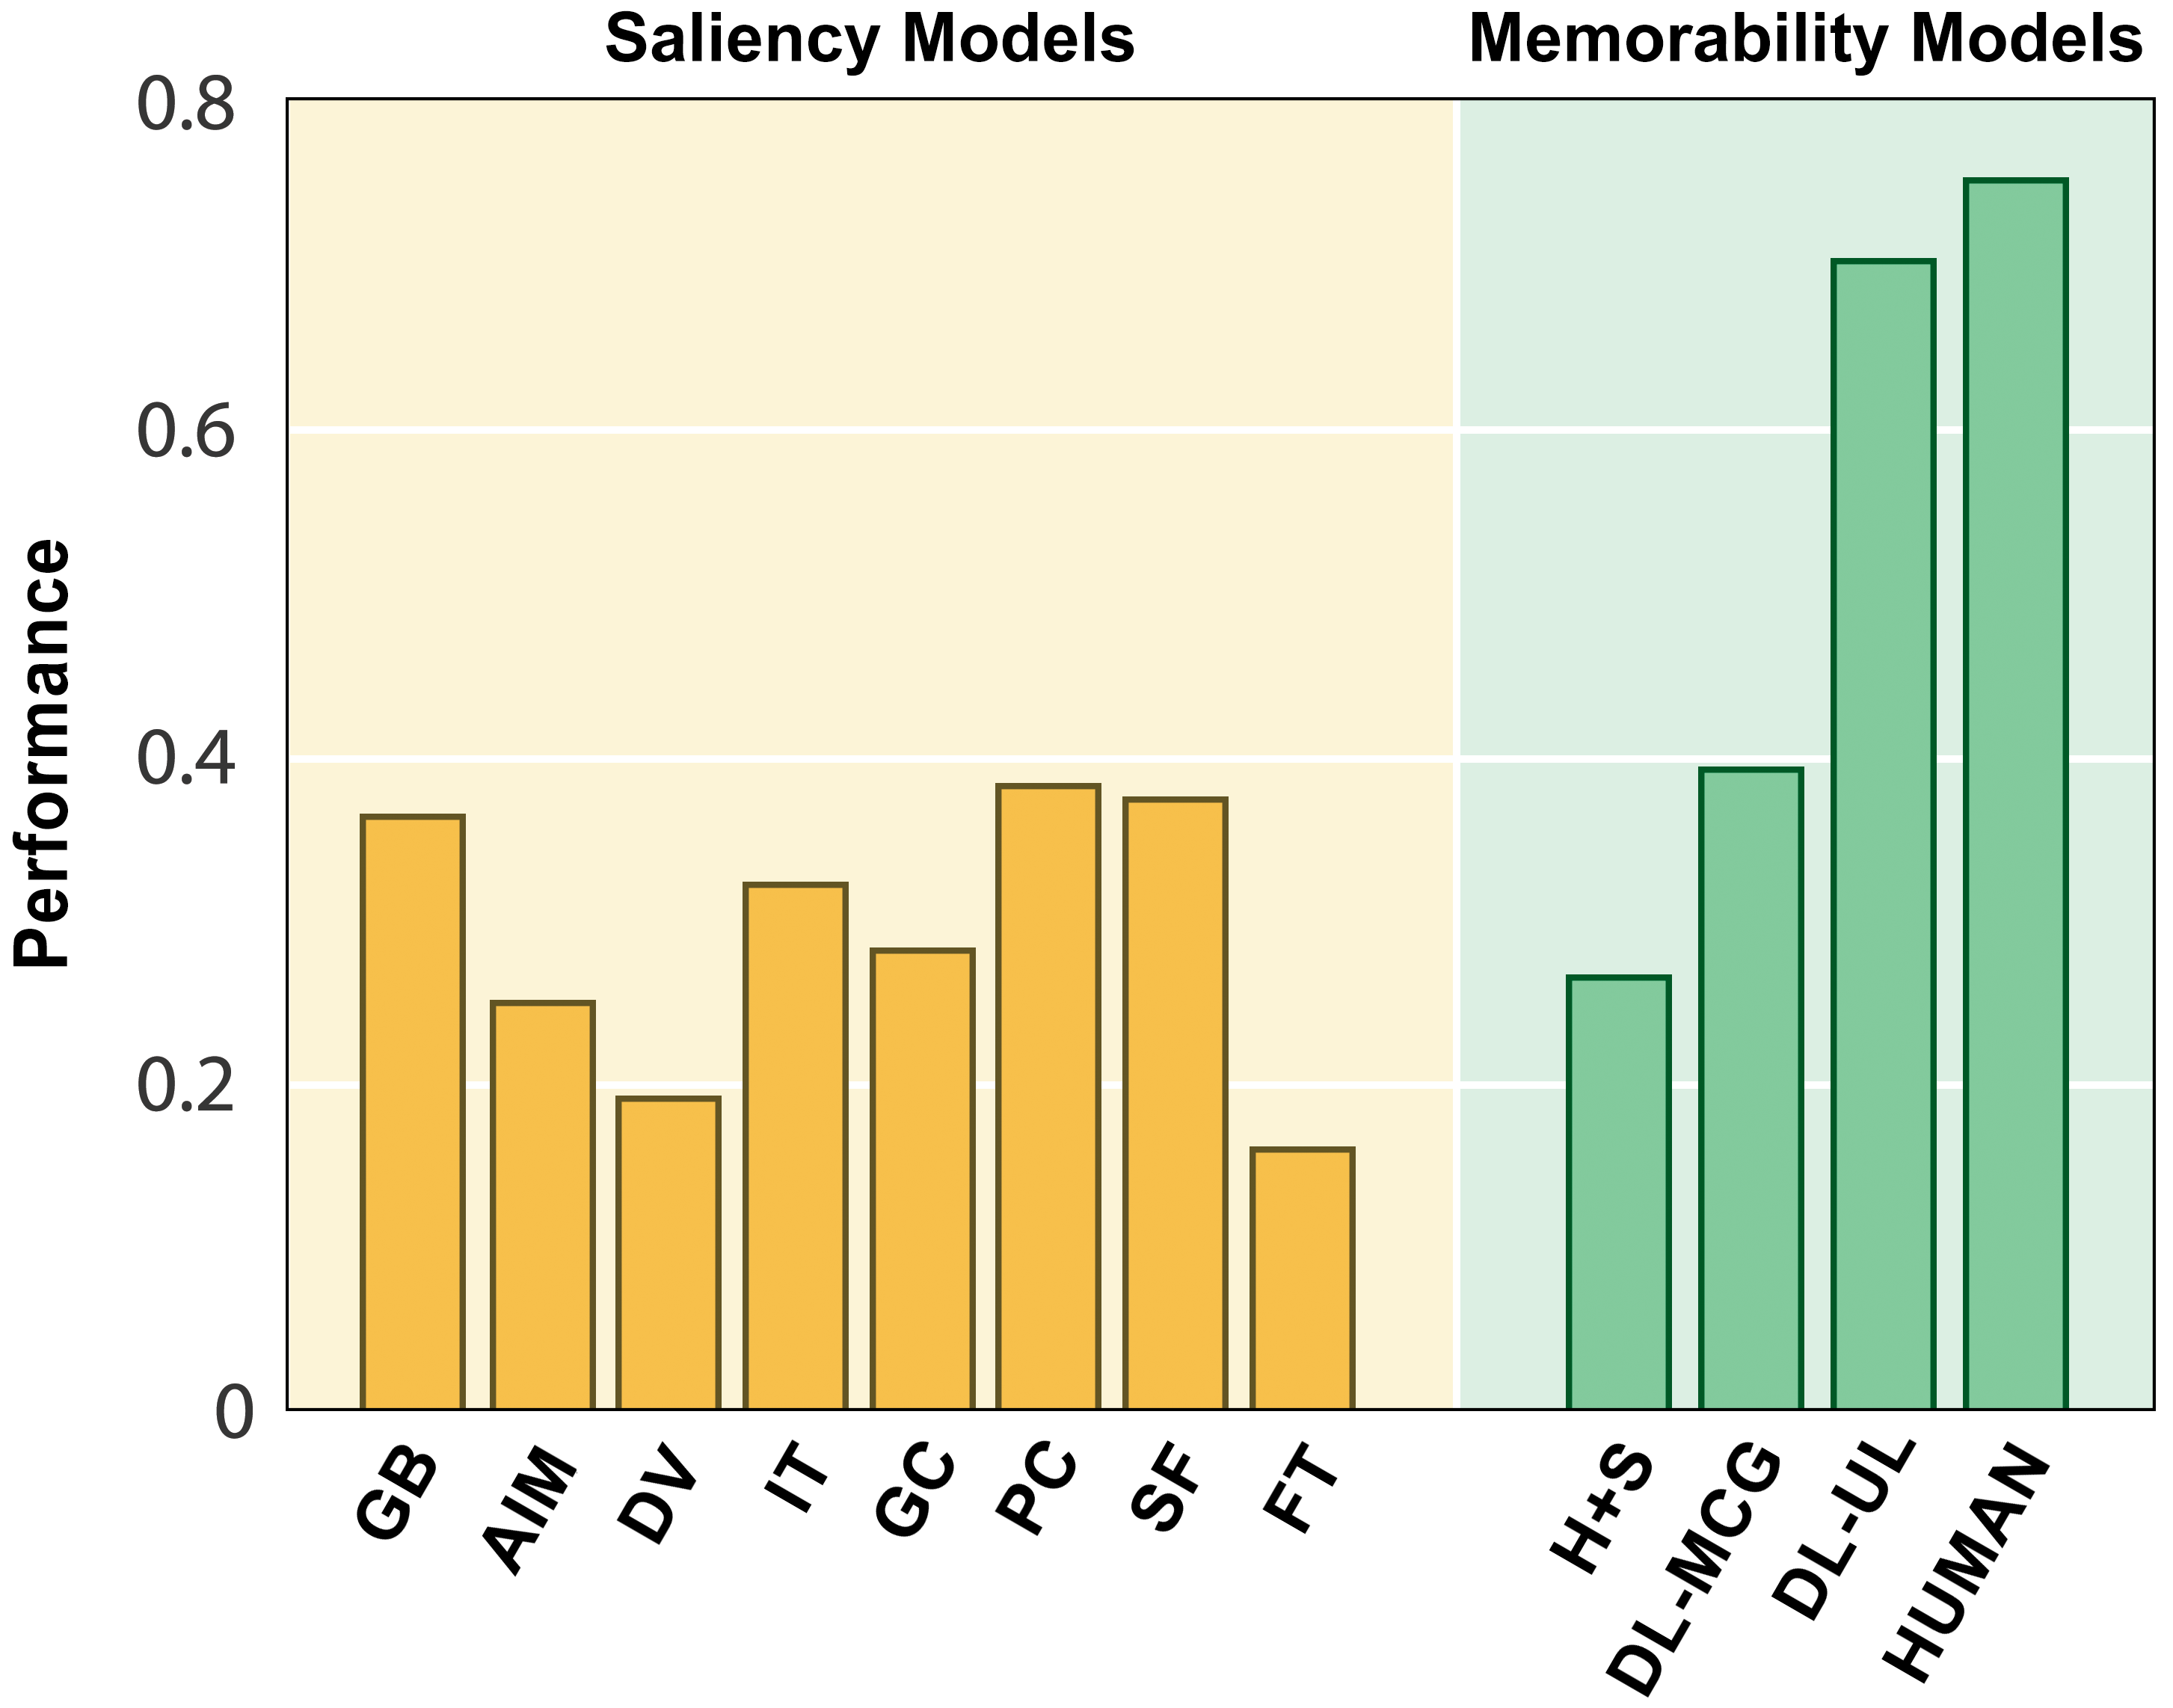
\includegraphics[width=0.4\textwidth]{figures/results/benchmark/comparison.png}}
\vspace{-5mm}\caption{\footnotesize\textbf{Main task.} add-in later. }\label{fig:benchmark}
\end{figure} 


{\small
\bibliographystyle{ieee}
\bibliography{egbib}
}

\end{document}
